\documentclass{article}
\usepackage{amsmath}
\usepackage{amssymb}
\usepackage{tcolorbox}
\usepackage{tikz}
\usepackage{geometry}
\geometry{a4paper, margin=1in}

\title{IB Analysis and Approaches HL2 \\ Inverse Trigonometric Functions}

\begin{document}
\maketitle

\section*{Introduction}
Inverse trigonometric functions are crucial for determining angles from given trigonometric ratios. They are the inverse operations of the basic trigonometric functions.

\section*{Understanding Trigonometry}
Suppose we have a right triangle with an angle $\theta$ and sides of length $a$, $b$, and $c$ as shown below.

\begin{center}
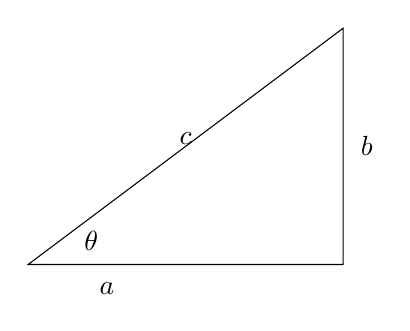
\begin{tikzpicture}
\draw (0,0) -- (4,0) -- (4,3) -- cycle;
\node at (1,-0.3) {$a$};
\node at (4.3,1.5) {$b$};
\node at (2,1.6) {$c$};
\node at (0.8,0.3) {$\theta$};
\end{tikzpicture}
\end{center}

In regular trigonometry:
\begin{align*}
\sin(\theta) &= \frac{b}{c}, \\
\cos(\theta) &= \frac{a}{c}, \\
\tan(\theta) &= \frac{b}{a}.
\end{align*}

\section*{Inverse Trigonometric Functions}
Inverse trigonometric functions return the angle for a given trigonometric ratio, essentially reversing the operations shown above.

\subsection*{Key Functions and Their Properties}
\begin{center}
\begin{tabular}{|c|c|c|c|}
\hline
Function & Definition & Domain & Range \\
\hline
$\arcsin(x)$ & $\sin(\arcsin(x)) = x$ & $-1 \leq x \leq 1$ & $-\frac{\pi}{2} \leq \arcsin(x) \leq \frac{\pi}{2}$ \\
$\arccos(x)$ & $\cos(\arccos(x)) = x$ & $-1 \leq x \leq 1$ & $0 \leq \arccos(x) \leq \pi$ \\
$\arctan(x)$ & $\tan(\arctan(x)) = x$ & $-\infty < x < \infty$ & $-\frac{\pi}{2} < \arctan(x) < \frac{\pi}{2}$ \\
\hline
\end{tabular}
\end{center}

\subsection*{Graphical Representations}
The graphs below help visualize the behavior and transformation from standard trigonometric functions to their inverses.

\begin{center}
\begin{tikzpicture}[scale=0.75]
% arcsin
\draw[->] (-4,0) -- (4,0) node[right] {$x$};
\draw[->] (0,-2) -- (0,2) node[above] {$y$};
\draw[domain=-1:1,smooth,variable=\x,blue] plot ({\x},{rad(asin(\x))});
\node at (4.5,-0.3) {\textcolor{blue}{$y = \arcsin(x)$}};

% arccos
\draw[->] (6,0) -- (14,0) node[right] {$x$};
\draw[->] (10,-1) -- (10,4) node[above] {$y$};
\draw[domain=-1:1,smooth,variable=\x,red] plot ({\x+10},{rad(acos(\x))});
\node at (14.5,-0.3) {\textcolor{red}{$y = \arccos(x)$}};

% arctan
\draw[->] (-4,-5) -- (4,-5) node[right] {$x$};
\draw[->] (0,-7) -- (0,-3) node[above] {$y$};
\draw[domain=-4:4,smooth,variable=\y,orange] plot ({\y},{rad(atan(\y))});
\node at (4.5,-5.3) {\textcolor{orange}{$y = \arctan(x)$}};
\end{tikzpicture}
\end{center}

\section*{Example Problems}
Here are some examples to practice:

1. \textbf{Calculate} $\arcsin(\frac{1}{2})$.
2. \textbf{Determine} $\arccos(-1)$.
3. \textbf{Find} $\arctan(1)$.

\end{document}
